\documentclass[10pt]{beamer}
\usepackage[many]{tcolorbox}

\usetheme{Copenhagen}

\definecolor{myblue1}{RGB}{35,119,189}
\definecolor{myblue2}{RGB}{95,179,238}
\definecolor{myblue3}{RGB}{129,168,207}
\definecolor{myblue4}{RGB}{26,89,142}

\setbeamercolor*{structure}{fg=myblue1,bg=blue}
\setbeamercolor*{palette primary}{use=structure,fg=white,bg=structure.fg}
\setbeamercolor*{palette secondary}{use=structure,fg=white,bg=structure.fg!75!black}
\setbeamercolor*{palette tertiary}{use=structure,fg=white,bg=structure.fg!50!black}
\setbeamercolor*{palette quaternary}{fg=black,bg=white}

\setbeamercolor*{item projected}{fg=red,bg=myblue3!80}
\setbeamercolor*{block title example}{fg=white,bg=myblue4}

\setbeamertemplate{blocks}[rounded][shadow=true]

\makeatletter
\defbeamertemplate*{frametitle}{mydefault}[1][left]
{
  \ifbeamercolorempty[bg]{frametitle}{}{\nointerlineskip}%
  \nointerlineskip%
  \@tempdima=\textwidth%
  \advance\@tempdima by\beamer@leftmargin%
  \advance\@tempdima by\beamer@rightmargin%
  \begin{tcolorbox}[
  enhanced,
  outer arc=0pt,
  arc=0pt,
  boxrule=0pt,
  top=0pt,
  bottom=0pt,
  enlarge left by=-\beamer@leftmargin,
  enlarge right by=-\beamer@rightmargin,
  width=\paperwidth,
  nobeforeafter,
  interior style={
    left color=myblue2,
    right color=white
    },
  shadow={0mm}{-0.4mm}{0mm}{black!60,opacity=0.6},    
  shadow={0mm}{-0.8mm}{0mm}{black!40,opacity=0.4},    
  ]
    \usebeamerfont{frametitle}%
    \vbox{}\vskip-1ex%
    \if@tempswa\else\csname beamer@fte#1\endcsname\fi%
    \insertframetitle\par%
    {%
      \ifx\insertframesubtitle\@empty%
      \else%
      {\usebeamerfont{framesubtitle}\usebeamercolor[fg]{framesubtitle}\insertframesubtitle\strut\par}%
      \fi
    }%
    \vskip-1ex%
    \if@tempswa\else\vskip-.3cm\fi% set inside beamercolorbox... evil here...
  \end{tcolorbox}%
}
\defbeamertemplate*{footline}{mysplit theme}
{%
  \leavevmode%
  \hbox{\begin{beamercolorbox}[wd=.5\paperwidth,ht=2.5ex,dp=1.125ex,leftskip=.3cm plus1fill,rightskip=.3cm]{author in head/foot}%
    \usebeamerfont{author in head/foot}\insertshortauthor
  \end{beamercolorbox}%
  \begin{beamercolorbox}[wd=.5\paperwidth,ht=2.5ex,dp=1.125ex,leftskip=.3cm,rightskip=.3cm plus1fil]{title in head/foot}%
    \usebeamerfont{title in head/foot}\insertshorttitle\hfill
    \insertframenumber/\inserttotalframenumber\hspace*{0.5em}
  \end{beamercolorbox}}%
  \vskip0pt%
}
\makeatother
\title{Le problème de transfert test github again}
\author{Gestion 2}
\date{\today}

\begin{document}
\begin{center}
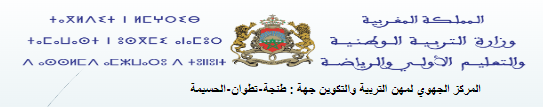
\includegraphics[scale=0.4]{logo.PNG} \\[0.1cm]
 \HRule \\[0.1cm]
  { \huge \bfseries 
  \textcolor{blue}{Gestion 2} \\[0.1cm]
  }
  \HRule 
  
  \HRule \\[0.1cm]
  { \huge \bfseries 
  \textcolor{black}{Le problème de transfert} \\[0.1cm]
  }
  \HRule 
  
\textsc{\alert{\Large 
 &Samady yassine \\[0.1cm]
 &Ismail mrabet\\[0.1cm]
 &Nahla tayibi\\[0.1cm]
 &Sagou mohamed\\[0.1cm]
 &Ben-abid saida\\[0.1cm]
 &Salma ayad el khalate\\[0.1cm]}}
 
\end{center}


\begin{frame}

\frametitle{Sommaire}
\tableofcontents[currentsection, hideothersubsections]

\end{frame}

\begin{frame}
\frametitle{\section{Le problème de transfert}}
\begin{block}{Définition }
Un problème de transfert en mathématiques est un type de problème qui implique le transfert de connaissances ou de compétences d'un domaine à un autre domaine. 
\end{block}
\end{frame}

\begin{frame}
\frametitle{\section{Les caractéristiques du problème de transfert }}
\begin{alertblock}{Les caractéristiques du problème de transfert}
•	La nécessité de transférer des connaissances.\\[0.3cm]
•	Le défi de la généralisation.\\[0.3cm]
•	La nécessité de la réflexion métacognitive.\\[0.3cm]
•	La variabilité des contextes.\\[0.3cm]
•	La nécessité de la créativité.\\[0.3cm]
•	La nécessité de la pratique.

\end{alertblock}

\end{frame}

\begin{frame}
\frametitle{\section{Application 1 :  Les mouvements plans }}
\begin{center}
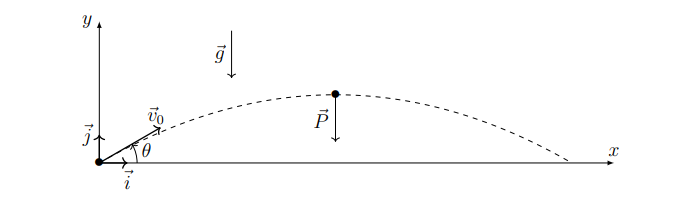
\includegraphics[scale=0.6]{9adifa.PNG}
\end{center}
\begin{block}{Application 1 }
On lance un projectile de masse m d’un point $O$ à l’instant $t = 0$ avec une vitesse initiale $\vec{v_{0}}$ qui fait un angle $\theta$ avec l’horizontale.
\end{block}
- Quel est Les équations horaires du mouvement et vitesse
\end{frame}

\begin{frame}
\begin{alertblock}{}
Les équations horaires du mouvement et vitesse :\\
Les composantes de $\vec{v_{0}}$ sont :
$$ \vec{v_{0}} \left\{
    \begin{array}{ll}
        v_{0x} = v_{0}.cos(\theta) \\ 
        v_{0y} = v_{0}.sin(\theta) 
    \end{array}
\right.$$
• Le système étudié est {Le projectile}.\\
• Le bilan des forces : Le projectile est soumis à son poids uniquement $\vec{P}$.\\
• D’après la deuxième loi de Newton on a :
\begin{align}
\sum \vec{F}  &= m\vec{a}\\
 \vec{P} &= m\vec{a}\\
  m\vec{g} &= m\vec{a}\\
  \vec{g} &= \vec{a} 
\end{align}
\end{alertblock}
\end{frame}

\begin{frame}
\begin{alertblock}{}
Projetons cette relation sur les axes :
$$

   \hspace{1.9cm}\left\{
    \begin{array}{ll}
        a_{x} = 0 \\ 
        a_{y} = -g 
    \end{array}
\right.  &\Leftrightarrow \left\{
    \begin{array}{ll}
        \dfrac{dv_{0x}}{dt} = 0 \\
        \dfrac{dv_{0y}}{dt} = -g
    \end{array}
    \right.\\[0.5cm]
    
 \hspace{3.8cm}  \vspace{0.5cm} &\Leftrightarrow  \left\{
    \begin{array}{ll}
        v_{x} = v_{0x} \\ 
        v_{y} = -gt + v_{0y} 
    \end{array}
    \right.
    
   
  \hspace{3.8cm} \vspace{0.5cm} &\Leftrightarrow  \left\{
    \begin{array}{ll}
        x = v_{0}.cos(\theta).t + x_{0} \\ 
        y = -\frac{1}{2}gt^{2} + v_{0}.sin(\theta).t + y_{0}
    \end{array}
    \right.
    
   \hspace{3.8cm} \vspace{0.5cm} &\Leftrightarrow  \left\{
    \begin{array}{ll}
        x = v_{0}.cos(\theta).t \\
        y = -\frac{1}{2}gt^{2} + v_{0}.sin(\theta).t
    \end{array}
\right. 
$$

\end{alertblock}
\end{frame}

\begin{frame}
\begin{alertblock}{}
Et ceux du mouvement sont :
$$\left\{
    \begin{array}{ll}
        x = v_{0}.cos(\theta).t \\[0.3cm]
        y = -\frac{1}{2}gt^{2} + v_{0}.sin(\theta).t
    \end{array}
\right.  $$

\end{alertblock}
\end{frame}

\begin{frame}
\frametitle{\section{Application 2 : La notion de centre de gravité en Physique }}
\begin{block}{Application 2 }
L’image ci-contre a été obtenu en filmant 5 images par secondes d’une solide lancée puis lâchée sur une table à coussin d’air horizontale immobile par rapport à la terre.
\end{block}
\begin{center}
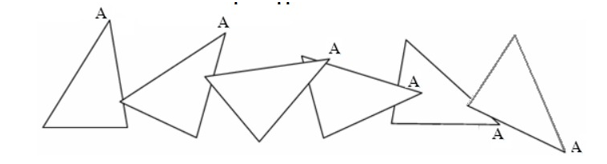
\includegraphics[scale= 0.5]{solide.PNG} 
\end{center}
\begin{block}{ }
1)	Quel est la trajectoire de la solide tout au long de la table ?\\
2)	Quelle est la vitesse moyenne de ce solide ? Quel est le type de ce mouvement ?
\end{block}
\end{frame}

\begin{frame}
\begin{alertblock}{}
1)	Pour déterminer la trajectoire de solide, on trace son centre de gravité (Intersection des médianes) dans les 5 images afin de les aligner.
\end{alertblock}
\begin{center}
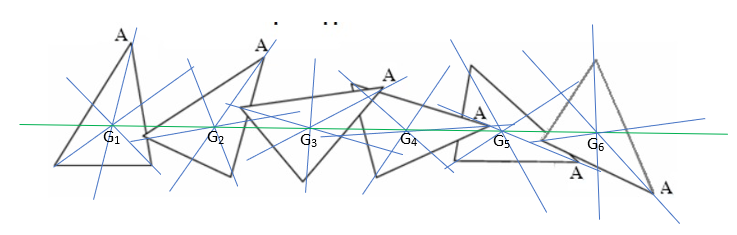
\includegraphics[scale=0.5]{solide 2.PNG} 
\end{center}
\end{frame}

\begin{frame}
\begin{alertblock}{}
2)	Pour calculer la vitesse moyenne, on mesure la distance $G_{1}G_{6}$ à l’aide de la règle en la divisant par la durée de filmage :
$$V_{moyennne} = \dfrac{G_{1}G_{6}}{6} = \frac{15}{6} = 2.5 m/s$$
On remarque que la distance entre 2 captures successive du centre de gravité est constante, et d’après la figure la trajectoire (en vert) est rectiligne. Donc le mouvement est rectiligne uniforme.
\end{alertblock}
\end{frame}


\begin{frame}
\frametitle{\section{Application 3 : Le travail d'une force en physique }}
\begin{block}{Application 3 }
On exerce sur un corps solide de force $\overrightarrow{F}$ constante d'intensité $\overrightarrow{F} = 200\text{ N}$ à l'aide d'un fil inextensible comme l'indique la figure suivante :
\end{block}

\begin{figure}[h]
\centering
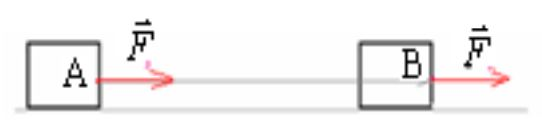
\includegraphics[width=0.4\textwidth]{figure1.jpg}
\end{figure}

\begin{block}{ }
Sachant que le corps se déplace d'un point $A$ à un point $B$ ($AB = 30\text{ m}$):\\
a)- Calculer le travail de la force $\overrightarrow{F}$ pendant ce déplacement.\\
b)- Même question si la force $\overrightarrow{F}$ forme un angle $\alpha = 20^\circ$ avec l'horizontale comme l'indique la figure suivante :
\end{block}

\begin{figure}[h]
\centering
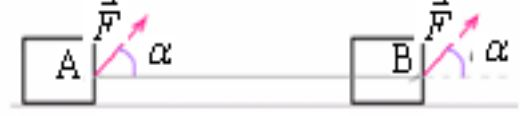
\includegraphics[width=0.4\textwidth]{figure2.JPG} 
\end{figure}
\end{frame}

\begin{frame}
\begin{block}{ }
c)- Quel serait l'angle $\alpha$ pour lequel la force $\overrightarrow{F}$ n'aurait aucun effet sur le déplacement de $A$ vers $B$? \\
d)- Supposons maintenant que la trajectoire $AB$ est inclinée (voir la figure). Justifier que le travail de la force $\overrightarrow{P}$ le poids du solide, est donné par la formule suivante :\\
\begin{equation*}
    W_{AB}(\overrightarrow{P}) = P\times H
\end{equation*} 
où $H$ est la différence d'altitude entre les points $A$ et $B$.
\end{block}
\begin{figure}[h]
\centering
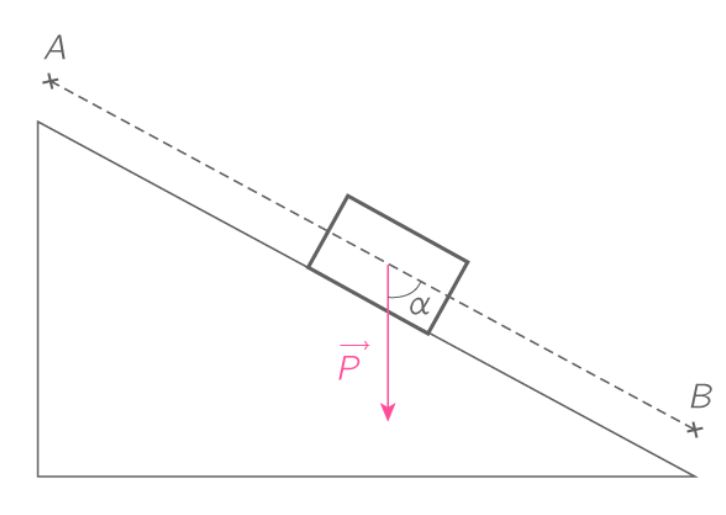
\includegraphics[width=0.4\textwidth]{figure3.jpg}
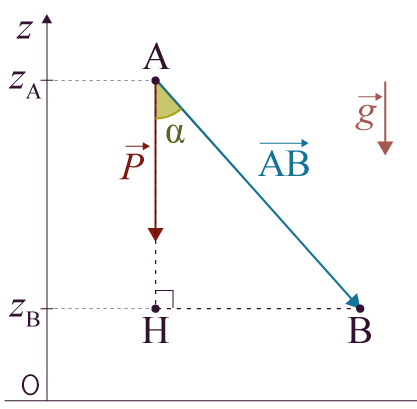
\includegraphics[width=0.3\textwidth]{figure4.png}
\end{figure}
\end{frame}


\begin{frame}
\textbf{Solution}
\begin{alertblock}{}
a)- Le travail de la force F est donné par la formule suivante :
\begin{equation*}
W_{AB}(\overrightarrow{F}) = \overrightarrow{F} \cdot \overrightarrow{AB} = F \cdot AB \cdot \cos\alpha
\end{equation*}
Où $F$ est l'intensité de la force, $AB$ est la distance parcourue et $\alpha$ est l'angle entre la force et la direction du déplacement.\\
Dans ce cas, $F = 200 \textbf{ N}$, $AB = 30 \textbf{ m}$ et $\alpha = 0^\circ$ (car la force est parallèle à la direction du déplacement).\\
Ainsi, le travail de la force F est,
\begin{align*}
    W_{AB}(\overrightarrow{F}) &= \overrightarrow{F} \cdot \overrightarrow{AB} \\
    & = F \cdot AB \cdot \cos\alpha \\ 
    &= 200 \times 30 \times \cos(0) \\
    &= \boxed{6000 \text{ J}}
\end{align*}
\end{alertblock}
\end{frame}
\begin{frame}
\begin{alertblock}{}
b)- Si la force $\overrightarrow{F}$ forme un angle $\alpha = 20^\circ$ avec l'horizontale, le travail de la force pendant le déplacement de $A$ à $B$ est donné par,
\begin{align*}
W_{AB}(\overrightarrow{F}) &= \overrightarrow{F} \cdot \overrightarrow{AB} \\
&= F \cdot AB \cdot \cos\alpha \\
&= 200 \times 30 \times \cos(20^\circ) \\
&\approx \boxed{5736 \text{ J}}
\end{align*}
\end{alertblock}
\end{frame}

\begin{frame}
\begin{alertblock}{}
c)- Si la force F n'aura aucun effet sur le déplacement de A vers B, Alors le travail W effectué par la force F sur A sera nul, c-à-d,
\begin{align*}
 \quad & W_{AB}(\overrightarrow{F}) = 0  \\
\Longleftrightarrow \quad &\overrightarrow{F} \cdot \overrightarrow{AB}=0 \\
\Longleftrightarrow \quad & F \cdot AB \cdot \cos\alpha = 0
\end{align*}
\noindent et puisque $F \neq 0$ et $AB \neq 0$ donc,
$\cos\alpha = 0$\\
Alors pour que la force $\overrightarrow{F}$ n’aurait aucun effet sur le déplacement de $A$ vers $B$, l'angle $\alpha$ entre la force et la direction du déplacement du solide, peuvent être égale à $\pi/2$ ou $-\pi/2$.
\end{alertblock}
\end{frame}

\begin{frame}
\begin{alertblock}{}
d)- D'après la définition on a, 
\begin{align*}
    W_{AB}(\overrightarrow{P}) &= \overrightarrow{P} \cdot \overrightarrow{AB} \\
    & = P \cdot AB \cdot \cos\alpha 
\end{align*}
\end{alertblock}

\begin{figure}[h]
\centering\
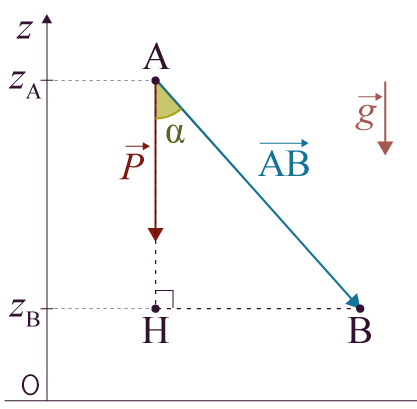
\includegraphics[width=0.3\textwidth]{figure4.png}
\end{figure}
\end{frame}

\begin{frame}
\begin{alertblock}{}
\noindent d'apés la figure,
\begin{align*}
 \quad & \cos\alpha = \frac{z_a-z_b}{AB} \\
\Longleftrightarrow \quad & AB = \frac{z_a-z_b}{\cos\alpha} 
\end{align*}

Donc, 
\begin{align*}
 \quad & W_{AB}(\overrightarrow{P}) =\dfrac{P.(z_a-z_b)}{cos(\alpha)}.cos(\alpha) \\
\Longleftrightarrow \quad & W_{AB}(\overrightarrow{P}) = P.(z_a-z_b) \\
\Longleftrightarrow \quad & \boxed{W_{AB}(\overrightarrow{P}) = P.H}
\end{align*}

\
où $H$ est la différence d'altitude entre les points $A$ et $B$.

\end{alertblock}
\end{frame}


\begin{frame}
\begin{figure}[h]
\centering

\includegraphics[width=0.6\textwidth]{merci.PNG} 
\end{figure}
\end{frame}


\end{document}
